\section{Thiết kế mạch trên Altium Design}

\subsection{Schematic}

\subsubsection{Design a 3.3V regulator}
\begin{figure}[!htbp]
    \centering
    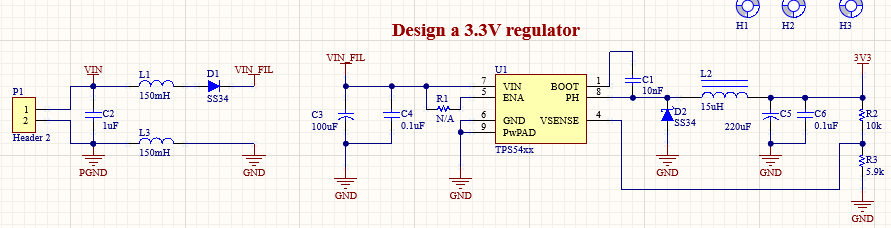
\includegraphics[width=\textwidth]{graphics/section3/f1.PNG}
\end{figure}

\subsubsection{Design a ESP32-WROM-32 part}
\begin{figure}[!htbp]
    \centering
    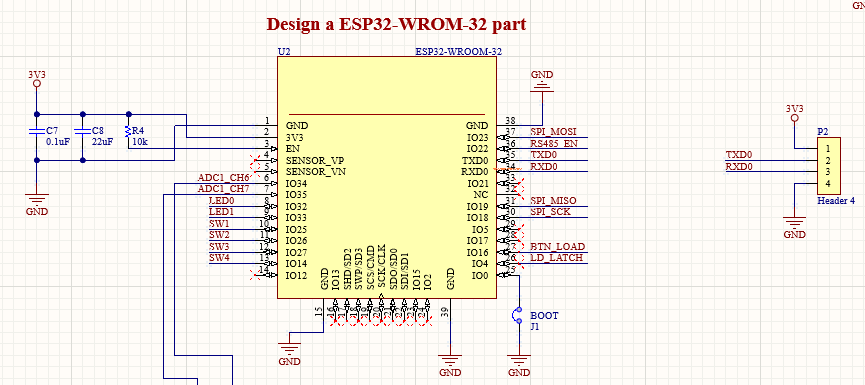
\includegraphics[width=\textwidth]{graphics/section3/f2.PNG}
\end{figure}

\subsubsection{Interfacing Slide Switch with an MCU}
\label{subsec: Interfacing Slide Switch with an MCU}
\begin{figure}[!htbp]
    \centering
    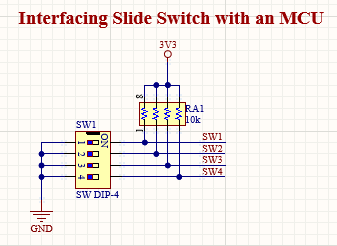
\includegraphics[width=0.3\textwidth]{graphics/section3/f3.PNG}
\end{figure}
\FloatBarrier

\subsubsection{Current sensor circuit}
\begin{figure}[!htbp]
    \centering
    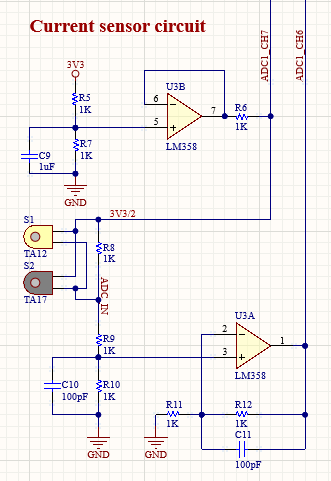
\includegraphics[width=0.3\textwidth]{graphics/section3/f4.PNG}
\end{figure}
\FloatBarrier

\subsubsection{Design a RS-485 part}
\begin{figure}[!htbp]
    \centering
    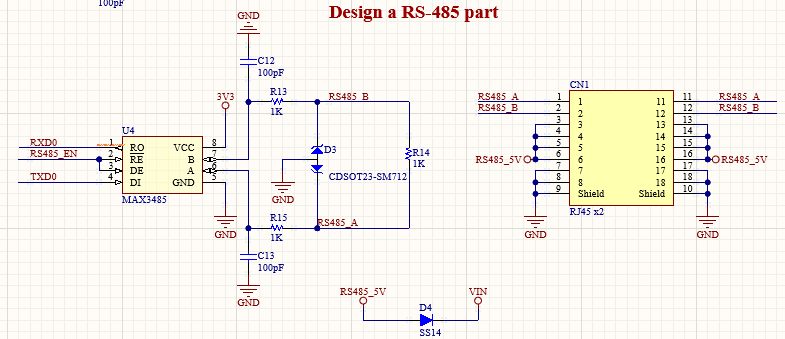
\includegraphics[width=\textwidth]{graphics/section3/f5.PNG}
\end{figure}
\FloatBarrier

\subsubsection{Interface with high-current LEDs}
\begin{figure}[!htbp]
    \centering
    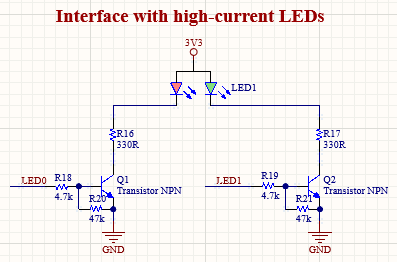
\includegraphics[width=0.7\textwidth]{graphics/section3/f6.PNG}
\end{figure}
\FloatBarrier

\subsection{PCB layout}
\begin{figure}[!htbp]
    \centering
    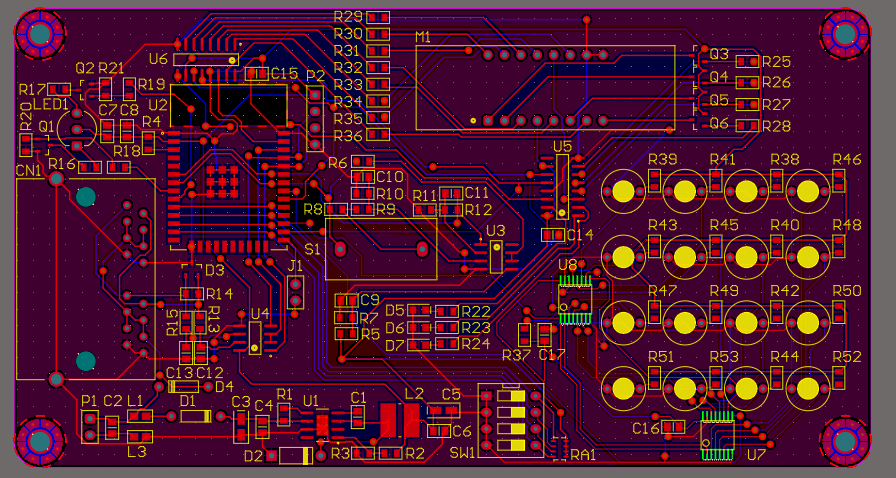
\includegraphics[width=\textwidth]{graphics/section3/f7.PNG}
    \caption{Top layer}
\end{figure}
\FloatBarrier

\begin{figure}[!htbp]
    \centering
    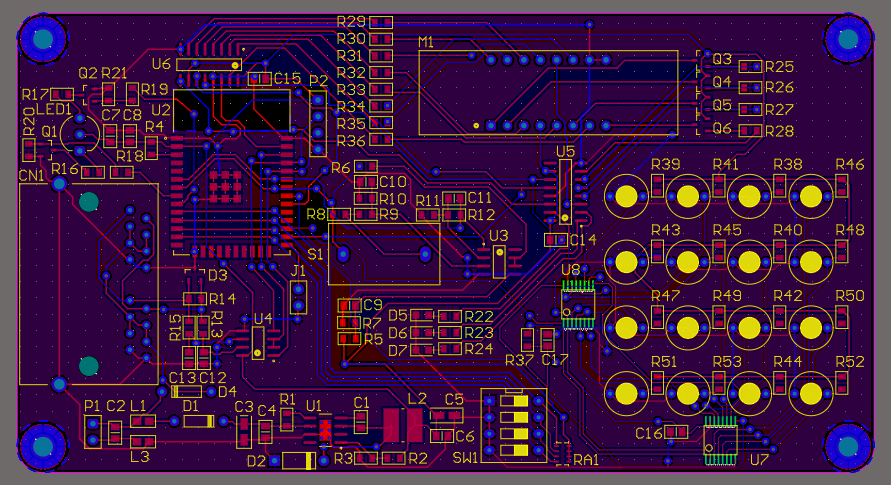
\includegraphics[width=\textwidth]{graphics/section3/f8.PNG}
    \caption{Bottom layer}
\end{figure}
\FloatBarrier
\subsection{Thành phẩm 3D}
\begin{figure}[!htbp]
    \centering
    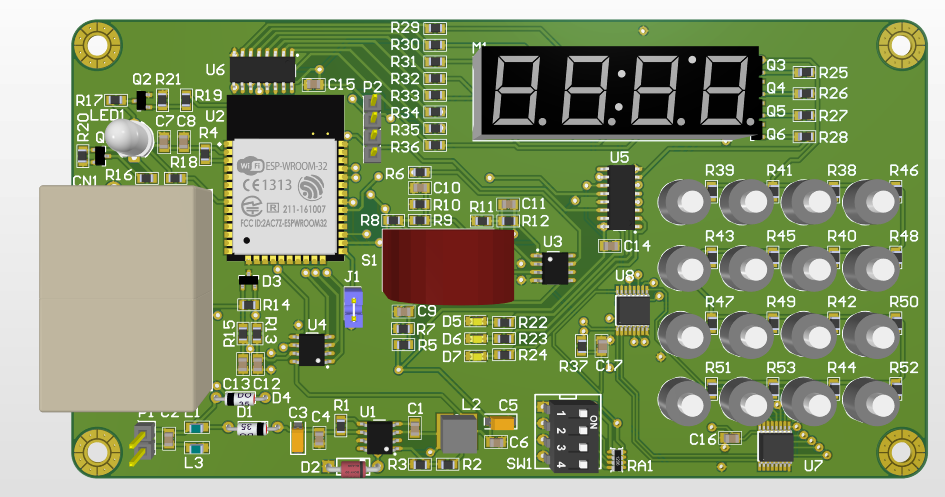
\includegraphics[width=\textwidth]{graphics/section3/f9.PNG}
    \caption{Top view}
\end{figure}
\FloatBarrier
\pagebreak
{ }
\begin{figure}[!htbp]
    \centering
    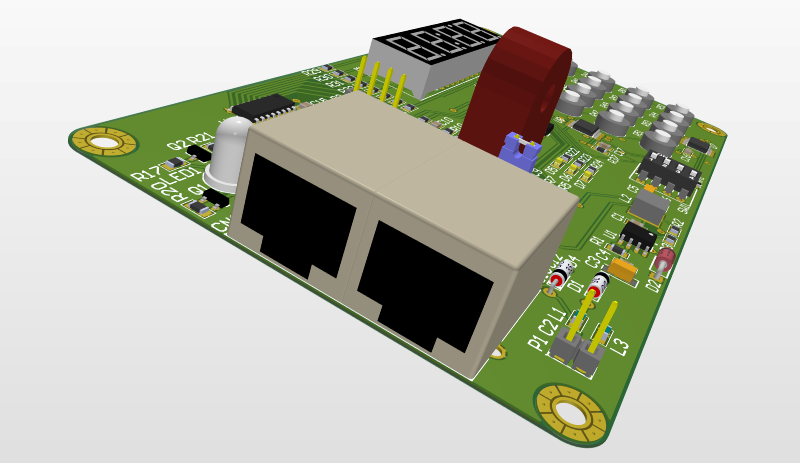
\includegraphics[width=\textwidth]{graphics/section3/f10.PNG}
    \caption{Isometric view}
\end{figure}
\FloatBarrier

